%%%%%%%%%%%%%%%%%%%%%%%%%%%%%%%%%%%%%%%%%%%%%%%%%%%%%%%%%%%%%%%%%%%%%%
% Lớp 8 | Chương III. Tứ giác | Hình bình hành
% Dạng 8H3?12-3: Chứng minh đoạn thẳng, góc bằng nhau, ba điểm thẳng hàng
%%%%%%%%%%%%%%%%%%%%%%%%%%%%%%%%%%%%%%%%%%%%%%%%%%%%%%%%%%%%%%%%%%%%%%


% nguồn: De_AI_Toan8_cuoi_hoc_ki_i_1 (nhập 21/11/2026)
\begin{bt}%[8H3H12-3]%[ma:4bdbca01]
	Cho hình bình hành $ABCD$ có $O$ là giao điểm của hai đường chéo $AC$ và $BD$. Một đường thẳng đi qua $O$ cắt cạnh $AB$ tại $M$ và cắt cạnh $CD$ tại $N$.
a) Chứng minh tam giác $OAM$ bằng tam giác $OCN$.
b) Chứng minh $OM = ON$ và $AM = CN$.
	\loigiai{
		a) Vì $ABCD$ là hình bình hành nên $O$ là trung điểm của $AC$ ($OA = OC$) và $AB \parallel CD$, suy ra $\widehat{OAM} = \widehat{OCN}$ (so le trong). \\
Xét $\triangle OAM$ và $\triangle OCN$ có: $\widehat{OAM} = \widehat{OCN}$, $OA = OC$, $\widehat{AOM} = \widehat{CON}$ (đối đỉnh). \\
Suy ra $\triangle OAM = \triangle OCN$ (g.c.g). \\
b) Từ $\triangle OAM = \triangle OCN$ suy ra $OM = ON$ và $AM = CN$ (các cặp cạnh tương ứng).
	}
\end{bt}

% nguồn: De_AI_Toan8_cuoi_hoc_ki_i_1 (nhập 21/11/2026)
\begin{bt}%[8H3H12-3]%[ma:5c75f205]
	Cho hình bình hành $ABCD$. Gọi $E$, $F$ lần lượt là trung điểm của các cạnh $AD$ và $BC$.
a) Chứng minh tứ giác $BEDF$ là hình bình hành, từ đó suy ra $BE = DF$.
b) Chứng minh ba đường thẳng $AC$, $BD$, $EF$ cùng đi qua một điểm.
	\loigiai{
		a) Vì $ABCD$ là hình bình hành nên $AD \parallel BC$ và $AD = BC$. \\
Vì $E$, $F$ là trung điểm $AD$, $BC$ nên $ED = \dfrac{1}{2}AD = \dfrac{1}{2}BC = BF$ và $ED \parallel BF$. \\
Suy ra tứ giác $BEDF$ là hình bình hành, do đó $BE = DF$. \\
b) Gọi $O$ là giao điểm hai đường chéo $AC$ và $BD$ của hình bình hành $ABCD$, suy ra $O$ là trung điểm của $BD$. \\
Vì $BEDF$ là hình bình hành có hai đường chéo là $BD$ và $EF$, nên hai đường chéo này cắt nhau tại trung điểm của mỗi đường. \\
Do $O$ là trung điểm của $BD$ nên $EF$ cũng đi qua $O$. Vậy $AC$, $BD$, $EF$ cùng đi qua điểm $O$.
	}
\end{bt}

% nguồn: De_AI_Toan8_cuoi_hoc_ki_i_1 (nhập 21/11/2026)
\begin{bt}%[8H3H12-3]%[ma:6376c0a3]
	Cho hình bình hành $ABCD$. Gọi $E$ là điểm đối xứng với $A$ qua $B$, $F$ là điểm đối xứng với $C$ qua $D$.
a) Chứng minh tứ giác $BEDF$ là hình bình hành.
b) Gọi $O$ là trung điểm của $BD$. Chứng minh ba điểm $E$, $O$, $F$ thẳng hàng.
	\loigiai{
		a) Vì $ABCD$ là hình bình hành nên $AB \parallel CD$ và $AB = CD$. \\
Vì $E$ đối xứng với $A$ qua $B$ nên $B$ là trung điểm $AE$, suy ra $BE = AB$ và $BE \parallel CD$. \\
Vì $F$ đối xứng với $C$ qua $D$ nên $D$ là trung điểm $CF$, suy ra $DF = CD$ và $DF \parallel AB$. \\
Từ đó $BE = DF$ và $BE \parallel DF$, nên tứ giác $BEDF$ là hình bình hành. \\
b) Trong hình bình hành $BEDF$, hai đường chéo $BD$ và $EF$ cắt nhau tại trung điểm của mỗi đường. \\
Vì $O$ là trung điểm của $BD$ nên $O$ cũng là trung điểm của $EF$, suy ra ba điểm $E$, $O$, $F$ thẳng hàng.
	}
\end{bt}

% nguồn: chuyen_dang (nhập 22/11/2026)
\begin{bt}%[BG12-3in1, Nguyễn Xuân Bảo-Phạm Ngọc Trung]%[8H3V12-3] % KIEM_TRA%[ma:052d0dfa]
Cho hình bình hành $ABCD$, chứng minh $AC^2+BD^2=2AC^2+2BD^2$.
	\loigiai{
	\immini{
	Áp dụng định lý côsin trong tam giác $ABD$, ta có $$BD^2=AB^2+AD^2-2AB\cdot AD \cos A.$$
	Áp dụng định lý côsin trong tam giác $ABC$, ta có $$AC^2=AB^2+BC^2-2AB \cdot BC \cos B.$$
		}
		{
			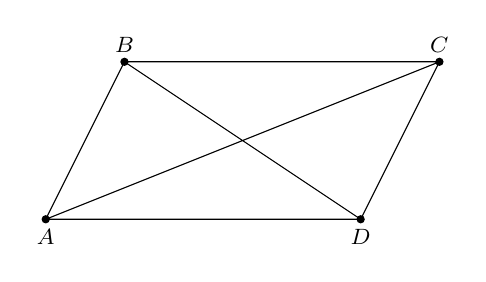
\begin{tikzpicture}[scale=1, font=\footnotesize, line join=round, line cap=round, >=stealth]
			\coordinate[label=below:$A$] (A) at (0,0);
			\coordinate[label=above:$B$] (B) at (1,2);
			\coordinate[label=above:$C$] (C) at (5,2);
			\coordinate[label=below:$D$] (D) at (4,0);	
			\draw (A)--(B)--(C)--(D)--(A)--(C) (D)--(B);
			\foreach \diem in {A,B,C,D}\fill (\diem)circle(1.5pt);
		\end{tikzpicture}
		}
		Mà $ABCD$ là hình bình hành nên ta có $BC=AD$ $\widehat{A}+\widehat{B}=180^\circ$ suy ra $\cos B =-\cos A$, do đó
	$$AC^2=AB^2+AD^2+2AB\cdot AD \cos A.$$
	Vậy $AC^2+BD^2=2AB^2+2AD^2$.
	}
\end{bt}
